\documentclass{article}
\usepackage[utf8]{inputenc}
\usepackage{latexsym}
\usepackage{amsmath}
\usepackage{amssymb}
\usepackage{amsfonts}       % blackboard math symbols
\usepackage{nicefrac}       % compact symbols for 1/2, etc.
\usepackage{microtype}      % microtypography
\usepackage{pgf}
\usepackage{apalike}
\setcounter{tocdepth}{3}
\usepackage{graphicx}
\usepackage{color}
\usepackage{paralist}
\usepackage{tikz}
\usepackage{xspace}
\usepackage{subcaption}
\usepackage{physics}
\usetikzlibrary{bayesnet}
\usepackage{comment}
\usepackage{cancel}
\usepackage{exercise}
\usepackage{amsthm}
%%%% hyperlinks
\usepackage{hyperref}
\definecolor{darkblue}{rgb}{0, 0, 0.5}
\hypersetup{colorlinks=true,citecolor=darkblue, linkcolor=darkblue, urlcolor=darkblue}
%%%%


% Headers
\newcommand{\reftab}[1]{Table~\ref{tab:#1}}
\newcommand{\refeq}[1]{Equation~\ref{eq:#1}}
\newcommand{\reffig}[1]{Figure~\ref{fig:#1}}
\newcommand{\refalg}[1]{Algorithm~\ref{alg:#1}}
\newcommand{\refsec}[1]{Section~\ref{sec:#1}}

% Notes
\newcommand{\todo}[1]{{\bf \color{red} [TODO }{\em #1}{\bf ]}}

% Brackets
\newcommand{\angbrack}[1]{\ensuremath{\langle #1 \rangle}}

% Dimensionality
\newcommand{\dx}{\ensuremath{{d_{\texttt{x}}}}}
\newcommand{\dhidden}{\ensuremath{{d_{\texttt{h}}}}}
\newcommand{\dz}{\ensuremath{{d_{\texttt{z}}}}}
\newcommand{\vx}{\ensuremath{{v_{\texttt{x}}}}}
\newcommand{\vy}{\ensuremath{{v_{\texttt{y}}}}}

% Operators and functions
\DeclareMathOperator{\KL}{KL}
\DeclareMathOperator{\ELBO}{ELBO}
\DeclareMathOperator{\softmax}{softmax}
\DeclareMathOperator{\softplus}{softplus}
\DeclareMathOperator{\diag}{diag}
\DeclareMathOperator{\onehot}{one-hot}
\DeclareMathOperator*{\argmin}{\arg\!\min}
\DeclareMathOperator*{\argmax}{\arg\!\max}

% Distributions
\DeclareMathOperator{\Cat}{Cat}
\DeclareMathOperator{\Bern}{Bern}

\newcommand{\Pa}{\ensuremath{\mathbf{\text{Pa}}}}
\newcommand{\pa}{\ensuremath{\mathbf{\text{pa}}}}

% Language codes
\newcommand{\Lx}{\texttt{L1}\xspace}
\newcommand{\Ly}{\texttt{L2}\xspace}




\title{Probabilistic Graphical Models}

\author{Wilker Aziz}


\begin{document}
\maketitle

Here I briefly describe some of the important results about graphical models that are necessary to follow my bachelor's course on natural language models and interfaces. For now, I only cover directed graphical models.

These notes are largely based on \href{https://homes.cs.washington.edu/~taskar/pubs/gms-srl07.pdf}{Graphical models in a nutshell}.


\paragraph{Notation}

We use capital Roman letters (e.g. $X$) for random variables (rvs) and lowercase letters for assignments (e.g. $x$). We use $X_1^n$ as a shorthand for $X_1, \ldots, X_n$ and similarly with $x_1^n$. 
We write $P_X$ for probability distributions, and $P_X(X=x)$ for probability values---where we sometimes omit one or both occurrences of $X$, e.g. $P_X(x)$, $P(X=x)$, or $P(x)$, if no ambiguity is possible. 
%We denote a probability mass function (pmf) by $p(x; \alpha)$, where $\alpha$ is a deterministic set of parameters. Throughout, we also assume that $\argmax$ returns a single point.

%Assume we have a dataset of $n$ iid observations $\mathcal D = \{x_1, \ldots, x_n\}$ of an rv $X \sim P_X$, i.e. $\left(X_i \sim P_X\right)_{i=1}^n$.
%First of all, from independence, we know that 
%\begin{equation}
%P_{X_1^n}(x_1, \ldots, x_n) = \prod_{i=1}^n P_{X_i}(x_i) = \prod_{i=1}^n P_{X}(x_i) 
%\end{equation}
%and we then model the probability $P_X(x)$ with a member $p(x; \alpha)$ of a parametric family  and proceed to derive a maximum likelihood estimate of $\alpha$.
%In the following sections we use $\mathcal L(\alpha|\mathcal D)$ for the $\log$-likelihood %function
%\begin{equation}
%\mathcal L(\alpha|\mathcal D) = \sum_{i=1}^n \log p(x_i; \alpha)
%\end{equation}
%and we often omit the dependency on data writing simply $\mathcal L(\alpha)$.
%Our objective is then
%\begin{equation}\label{eq:mle}
%\theta^\star = \argmax_{\theta \in \Theta} ~ \mathcal L(\theta) 
%\end{equation}
%where the space of valid parameters $\Theta$ is possibly subject to constraints.


\newpage
I focus on discrete probability distributions with finite support throughout.
We start with the class of \emph{directed graphical models}, also known as \emph{Bayesian networks}. 


\section{Directed graphical models}


At the highest level our goal is to efficiently represent a joint distribution $P_{X_1,\ldots,X_n}$ over some collection of random variables $X_1, \ldots, X_n$.
Before we talk about \emph{efficient} ways of representing it, let's have a look at what it means to represent it \emph{inefficiently}.
If no simplifying assumptions can be made, the only way to represent the complete joint distribution is to use a table to store each probability value in its support. 
The support of the distribution is the set of all possible values its random variables may take on. 

For example, suppose that $X_i$ is a binary random variable---each $X_i$ can only take on 1 of 2 values. This means that altogether the collection $X_1, \ldots, X_n$ can take on $2^n$ different values. If we represent the joint distribution by storing the probability value associated with each and every joint outcome of $X_1, \ldots, X_n$, then we will need $2^n$ probability values.\footnote{More precisely, it takes $2^n - 1$ independent probability values, this is because probability values are positive and sum to 1, thus we can determine the last value by computing 1 minus the sum of probabilities of all other values. If asked about the representation cost of this example, I take any of the following as correct: $O(2^n)$, $2^n$, or $2^n -1$.}
This representation is called \emph{tabular}, since we can think of the distribution as a big table as in Table \ref{tab:3binary}.

\begin{table}[h]\centering
\begin{tabular}{c c c | c}
\multicolumn{3}{c|}{Joint assignments} & Probability values \\ 
$X_1$ & $X_2$ & $X_3$ & $P_{X_1, X_2, X_3}$ \\ \hline
0     &  0    &  0  & $P_{X_1, X_2, X_3}(0, 0, 0)$\\
0     &  0    &  1  & $P_{X_1, X_2, X_3}(0, 0, 1)$\\
0     &  1    &  0  & $P_{X_1, X_2, X_3}(0, 1, 0)$\\
1     &  0    &  0  & $P_{X_1, X_2, X_3}(1, 0, 0)$\\
0     &  1    &  1  & $P_{X_1, X_2, X_3}(0, 1, 1)$\\
1     &  1    &  0  & $P_{X_1, X_2, X_3}(1, 1, 0)$\\
1     &  0    &  1  & $P_{X_1, X_2, X_3}(1, 0, 1)$\\
1     &  1    &  1  & $P_{X_1, X_2, X_3}(1, 1, 1)$ \\ 
\end{tabular}
\caption{\label{tab:3binary}Example of tabular joint distribution over 3 binary random variables}
\end{table}

%Suppose we use a big table $\theta$ to store the probability values, and suppose we can index this table to refer to a particular value, i.e., $\theta_{x_1,x_2,x_3}$ refers to $P(X_1=x_1, X_2=x_2, X_3=x_3)$.

In the general case, where $\mathcal X_i$ is the support of the $i$th random variable, and $|\mathcal X_i|$ its size, the space of joint assignments will grow proportional to $\prod_{i=1}^n |\mathcal X_i|$, and that's the cost of our representation---one real number per joint assignment.

\begin{Exercise}[label=ABC]
Suppose $A$ may take on 1 out of $n$ values, $B$ may take on 1 out of $nm$ values, and $C$ is a binary variable. What's the representation cost of the joint distribution $P_{A,B,C}$ in the general case?
\end{Exercise}

~

A key concept in deriving compact representations of joint distributions is that of \emph{conditional independence}. 
Conditional independence relates 3 collections of random variables, e.g. $\mathbf X, \mathbf Y, \mathbf Z$ where we use boldface to denote a collection. If $\mathbf X \perp \mathbf Y | \mathbf Z$ ---which we read as $\mathbf X$ \emph{is conditionally independent of} $\mathbf Y$ \emph{given} $\mathbf Z$ --- then it holds that
\begin{equation}\label{eq:cond-ind}
P(\mathbf X, \mathbf Y| \mathbf Z) = P(\mathbf X|\mathbf Z) P(\mathbf Y| \mathbf Z)
\end{equation}
and by extension it also holds that
\begin{equation}\label{eq:cond-ind2}
P(\mathbf X| \mathbf Z, \mathbf Y) = P(\mathbf X|\mathbf Z)  ~ .
\end{equation}


\begin{Exercise}[label=cond-ind]
Prove that conditional independence (\ref{eq:cond-ind}) implies (\ref{eq:cond-ind2}).
\end{Exercise}

~

A directed graphical model, or a Bayesian network (BN), is a directed acyclic graph (DAG) $\mathfrak G$, where nodes represent random variables and  edges correspond to \emph{direct influence} of one node on another. 
You may think of a directed graphical model as a recipe to compactly represent a complex joint distribution. The compression in representation is due to the graphical model specifying a \emph{factorisation} of the joint distribution, that is, a way of building it \emph{a factor at a time}.

Let $\mathfrak G$ be a directed graphical model over the variables $X_1, \ldots, X_n$, then each random variable $X_i$ (and therefore each node of the graph)  has an associated \emph{conditional probability distribution} (cpd). A cpd fully specify the dependency of a random variable on other variables.
In particular, the cpd for the $i$th variable $X_i$ represents the probability of assignments to $X_i$ given assignments to parents of $X_i$ in $\mathfrak G$. The set of \emph{parents} of the $i$th variable is the set of all random variables that are directly connected to $X_i$---where the arrow points from the parent to $X_i$. We denote the set of parents by $\Pa_{X_i}$.  %---a random variable may have multiple parents thus we employ boldface to denote a collection. 

\begin{figure}[h]\centering
	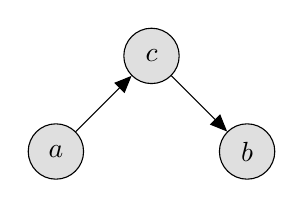
\begin{tikzpicture}
		% Define nodes
		\node[obs]	                (c)		{$ c $};
		\node[obs, below left= of c]	    (a)		{$ a $};
		\node[obs, below right= of c]     (b)     {$ b $}; 
		\edge{a}{c};
		\edge{c}{b};
	\end{tikzpicture}
	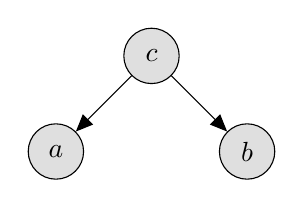
\begin{tikzpicture}
		% Define nodes
		\node[obs]	                (c)		{$ c $};
		\node[obs, below left= of c]	    (a)		{$ a $};
		\node[obs, below right= of c]     (b)     {$ b $}; 
		\edge{c}{a,b};
	\end{tikzpicture}
	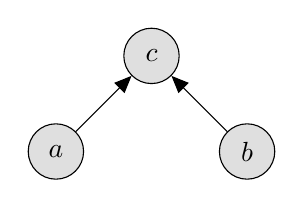
\begin{tikzpicture}
		% Define nodes
		\node[obs]	                (c)		{$ c $};
		\node[obs, below left= of c]	    (a)		{$ a $};
		\node[obs, below right= of c]     (b)     {$ b $}; 
		\edge{a,b}{c};
	\end{tikzpicture}
\caption{\label{fig:BN} Examples of directed graphical models}
\end{figure}

Figure \ref{fig:BN} illustrates three different BNs involving the same three random variables. For the first BN, on the left, 
\begin{itemize}
	\item $A$ has no parents, i.e., $\Pa_{A} = \emptyset$;
	\item $C$ has a single parent, i.e., $\Pa_C = \{A\}$;
	\item $B$ too has a single parent, i.e., $\Pa_B = \{C\}$.
\end{itemize}
For the second BN, in the middle, 
\begin{itemize}
	\item $C$ has no parents, i.e. $\Pa_C = \emptyset$;
	\item $A$ and $B$ both have the same (single) parent $C$, i.e., $\Pa_A = \Pa_B = \{C\}$.
\end{itemize}
Finally, for the last BN, on the right, 
\begin{itemize}
	\item $A$ and $B$ have no parents, i.e. $\Pa_A = \Pa_{B} = \emptyset$;
	\item $C$ has two parents, i.e., $\Pa_C = \{A, B\}$.
\end{itemize}

A cpd is a \emph{local probabilistic model}, that is, it is a probabilistic graphical model on its own right, but a small one that only explains a single variable. 
There are several ways to represent cpds, but for now we are only interested in the \emph{tabular} representation. The idea is exactly the same as we saw earlier, we will use a table of probability values per assignment in order to represent the conditional distribution. 

Consider an example where students' grades from $0$ to $10$ are mapped to a 3-class outcome (e.g. fail, pass, pass with honours), and consider whether or not I give the student a recommendation letter (a binary decision).\footnote{Example adapted from Daphne Koller's course on probabilistic graphical models.} 
Table \ref{tab:cpds} (right) illustrates the set of cpds associated with the variable letter $L$ given the variable grade $G$.
Note that to each outcome $G=g$ we associate a conditional probability distribution over $L$, that is, we have a probability value associated with each outcome in the support of $L$ and they sum to 1. In other words, every row in the tabular cpd is itself a distribution and we have as many cpds as there are values in the support $\mathcal G$ of $G$---exactly 3 in this case. Each cpd is itself a distribution over the support of $L$ and, in this example, contains 2 probability values. This means that it takes $3 \times 2$ probability values (or $3 \times (2-1)$ independent probability values) to represent the complete set of cpds $P_{L|G}$.
Table \ref{tab:cpds} (left) shows the cpd for $P_G$---you can think of it as a cpd that does not condition on anything (or conditions on the empty set)---note that the cpd sums to 1 as it should. 

\begin{table}[h]\small\centering
	\begin{tabular}{c c}
	\multicolumn{2}{c}{} \\
	Grade ($G$) & $P_G$ \\ \hline
	1 & 0.2 \\ 
	2 & 0.7 \\
	3 & 0.1 \\
	\multicolumn{2}{c}{} 
	\end{tabular}
	\qquad
	\begin{tabular}{l c | c c | c }
	Conditioning context &          & \multicolumn{2}{c|}{Letter ($L$)} & \\  
	Grade & $G$          & 0  & 1      &   $\sum_{l=0}^1 P_{L|G}(l|g)$  \\ \hline
	$[0, 6)$ & 1         & 0.8 & 0.2   & 1.0    \\
	$[6, 8)$ & 2         & 0.6 & 0.4   & 1.0     \\
	$[8, 10]$      & 3   & 0.1 & 0.9   & 1.0     \\
	\multicolumn{5}{c}{}
	\end{tabular}
	\caption{\label{tab:cpds}CPDs for $P_G$ (left) and $P_{L|G}$ (right).}
\end{table}

Recall that we can use chain rule to recover the complete joint distribution $P_{GL}$ over assignments to $G$ and $L$. That is, from chain rule $P_{GL}(g, l) = P_G(g)P_L(l|g)$.
Figure \ref{fig:joint-GL} (left) shows the complete joint distribution obtained by application of chain rule. 
\begin{figure}[h]\small\centering
	\begin{tabular}{c | c | c}
	\multicolumn{2}{c|}{Joint assignments} &  \\  
	$G$  & $L$   & $P_{GL}$ \\ \hline
	1    & 0     & 0.16 \\
	2    & 0     & 0.42 \\
	3    & 0     & 0.01 \\
	1    & 1     & 0.04 \\
	2    & 2     & 0.28 \\
	3    & 3     & 0.09 
	\end{tabular}
	~
	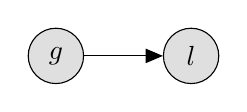
\begin{tikzpicture}
		% Define nodes
		\node[obs]	                (g)		{$ g $};
		\node[obs, right= of g]     (l)     {$ l $}; 
		\edge{g}{l};
	\end{tikzpicture}
	\caption{\label{fig:joint-GL}Joint distribution $P_{GL}$.}
\end{figure}
Note that while $P_G$ and $P_{L|G}$ are explicitly represented---they are stored in tables---the joint distribution $P_{GL}$ is \emph{inferred} by application of chain rule.
In other words, chain rule combines the \emph{marginal} $P_G$ with the conditionals $P_{L|G}$ to produce the joint $P_{GL}$.

The example just illustrated in fact corresponds to a very simple BN, shown in Figure \ref{fig:joint-GL} (right). The BN factorises the joint distribution using two factors---$P_G$ and $P_{L|G}$---which correspond to $4$ cpds (one for $P_G$, one for $P_{L|G=1}$, one for $P_{L|G=2}$, and one for $P_{L|G=3}$). 
Let's now think about the representation cost. $P_G$ takes $3-1=2$ independent probability values, and $P_{L|G}$ takes $3 \times (2-1) = 3$ independent probability values, thus our representation of the joint distribution---indirectly via chain rule---takes $2 + 3=5$ independent probability values. 
It does not look like we achieved much, since without assuming a particular factorisation we would expect $P_{GL}$ to take $3\times 2 - 1=5$ independent probability values anyway. 
The benefits, however, will become clear as we add more and more random variables.


The next result, known as the \emph{BN chain rule}, is the most important result concerning BNs. 
Given a BN $\mathfrak G$, the joint probability $P_{X_1, \ldots, X_n}(x_1, \ldots, x_n)$ factorises as a product
\begin{align}\label{eq:BN-chain-rule}
P_{X_1, \ldots, X_n}(x_1, \ldots, x_n) &= \prod_{i=1}^n P(X=x_i|\Pa_{X_i}=\pa_{X_i}) 
\end{align}
where $\Pa_{X_i}$ denotes the set of parents of $X_i$ in $\mathfrak G$ and $\pa_{X_i}$ are assignments to those parents. This result also implies that $\mathbf X \perp \text{NonDescendants}_{\mathbf X} \mid \Pa_{\mathbf X}$ where $\mathbf X$ is any subset of the variables in the BN, $\Pa_{\mathbf X}$ the union of their parents, and $\text{NonDescendants}_{\mathbf X}$ the union of variables that do not descend from variables in $\mathbf X$.
%it states that the joint distribution over $X_1, \ldots, X_n$ factorises as shown on the right-hand side. Each 

Now with definition (\ref{eq:BN-chain-rule}) in mind, let's get back to the BNs in Figure (\ref{fig:BN}).
The first BN (left) implies that the joint distribution factorises as 
\begin{equation}\label{eq:BN1}
P_{ABC}(a,b,c) = P_A(a)P_{C|A}(c|a)P_{B|C}(b|c) ~ .
\end{equation}
The second BN (middle) implies the factorisation 
\begin{equation}\label{eq:BN2}
P_{ABC}(a,b,c) = P_C(c)P_{A|C}(a|c)P_{B|C}(b|c) ~ .
\end{equation}	
And finally, the third BN (right) factorises the joint distribution as 
\begin{equation}\label{eq:BN3}
P_{ABC}(a,b,c) = P_A(a)P_B(b)P_{C|AB}(c|a,b) ~ .
\end{equation}

Table \ref{tab:cost} shows the representation cost for the different cpds in Figure \ref{fig:BN} assuming that $A$ is ``one of $n$'', $B$ is ``one of $m$'', and $C$ is binary.
Recall that a general joint distribution $P_{ABC}$, if no independence assumptions can be made, takes $O(n \times m)$ parameters to represent (because there are $2 \times n \times m$ unique joint assignments). 
With the conditional independence assumptions in each of the BNs in Figure \ref{fig:BN}, we achieve different representation costs. 
For example, (\ref{eq:BN1}) takes $O(n + m)$, (\ref{eq:BN2}) also takes $O(n + m)$, but (\ref{eq:BN3}) takes $O(n \times m)$.
The reason why the last BN is not asymptotically more compact than the complete joint distribution is because it still correlates all $3$ variables directly through $P_{C|AB}$.
The other two BNs introduce stronger assumptions, for example by never correlating more than 2 variables at a time. 
	
\begin{table}[h]\centering
\begin{tabular}{l l l}
Distribution & \# joint assignments & Representation cost \\ \hline
$P_A$ & $n$ & $O(n)$ \\ 
$P_B$ & $m$ & $O(m)$ \\
$P_C$ & $2$ & $O(1)$ \\
$P_{A|C}$ & $2\times n$ & $O(n)$ \\
$P_{C|A}$ & $n \times 2$ & $O(n)$ \\
$P_{B|C}$ & $2 \times m$ & $O(m)$ \\
$P_{C|B}$ & $m \times 2$ & $O(m)$ \\
$P_{C|AB}$ & $n \times m \times 2$ & $O(n \times m)$
\end{tabular}
\caption{\label{tab:cost}Representation cost for cpds in Figure \ref{fig:BN} assuming $\mathcal A=\{1, \ldots, n\}$, $\mathcal B =\{1, \ldots, m\}$, and $\mathcal C =\{0, 1\}$.}
\end{table}
	
	
\subsection{Inferences}	

Equation (\ref{eq:BN-chain-rule}) shows us how to construct the joint distribution out of the cpds specified in a BN.
However, we may be interested in other quantities as well, such as marginals and conditionals that are not directly stored in cpds. 
For that, we start from the joint distribution---taking into account the particular factorisation---and proceed by applying standard rules of probability, such as, marginalisation, conditioning, and Bayes rule. 

For example, the BN in Figure \ref{fig:BN} (left) implies that we only have $P_A$, $P_{C|A}$, and $P_{B|C}$ stored as tabular cpds. However, we may be interested in computing the marginal distribution $P_B$, or the marginal $P_C$, or a conditional such as $P_{A|B}$ or $P_{B|A}$.
Let's illustrate this by computing the marginal distribution $P_B$.
\begin{subequations}
\begin{align}
\intertext{We start from the BN chain rule}
P_{ABC}(a,b,c) &= P_A(a)P_{C|A}(c|a)P_{B|C}(b|c) \\
\intertext{then we proceed to marginalise $A$}
P_{BC}(b,c) &= \sum_{a=1}^n P_A(a)P_{C|A}(c|a)P_{B|C}(b|c) \\
\intertext{then note that the last factor $P_{B|C}$ does not depend on $a$, thus we can factor it out (read ``push it outside'') of the sum}
 &= P_{B|C}(b|c) \sum_{a=1}^n P_A(a)P_{C|A}(c|a) \\
\intertext{then we may proceed to marginalise $C$}
P_B(b) &= \sum_{c=0}^1 P_{B|C}(b|c) \left(\sum_{a=1}^n P_A(a)P_{C|A}(c|a) \right) \label{eq:PB}
\end{align}
\end{subequations}
Note that every cpd in the final expression is a tabular cpd for which we can look probability values up directly.
Also note that inferring the marginal distribution $P_B$ requires performing the computation in (\ref{eq:PB}) $m$ times, that is, once per valid assignment of $B$, and therefore the overall computation runs in time proportional to $O(m \times 2 \times n) = O(n \times m)$---assuming we can look up probability values in constant time---even though we reduced the representation cost of the underlying joint distribution to $O(n+m)$.

If inferring marginals and conditionals may still essentially take $O(n \times m)$, why do we bother? 
The answer has to do with \emph{learning}. 
When we rely on parameter estimation derived from observations in order to choose the precise probability values that make up our various tabular cpds (i.e. $P_A$, $P_{C|A}$, and $P_{B|C}$), we need to be cautious with sparsity.
If we do not make assumptions, we will be left with enormous tabular cpds, and we will simply not find enough data to estimate their parameters.
Also, some assumptions are actually extremely reasonable and convey knowledge about the problem we are interested in. 
In fact, we can see probabilistic graphical models as a general framework to express our domain knowledge in terms of probability theory.

~

\begin{Exercise}[label=ABC]
For the BN in Figure \ref{fig:exBN1}, write down the joint distribution $P_{ABC}$, the conditional $P_{BC|A}$ and the conditional $P_{C|A}$. Your expressions must all be a function of the tabular cpds in the BN. 
Also state the representation cost of the joint distribution as a function of the size of the support of each variable: $n_a = |\mathcal A|$, $n_b = |\mathcal B|$, and $n_c = |\mathcal C|$. %And finally, for inferred distributions, state the algorithmic complexity.
\begin{figure}[h]\centering
	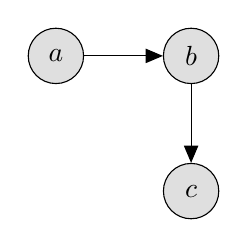
\begin{tikzpicture}
		% Define nodes
		\node[obs]	                 (a)		{$ a $};
		\node[obs, right = of a]	 (b)		{$ b $};
		\node[obs, below = of b]     (c)     {$ c $}; 
		\edge{a}{b};
		\edge{b}{c};
	\end{tikzpicture}
	\caption{\label{fig:exBN1}}
\end{figure}
\end{Exercise}

		
~

\begin{Exercise}[label=A-G]
For the BN in Figure \ref{fig:exBN2}, write down the joint distribution $P_{ABCDEFG}$ and the conditional $P_{FG|ABCDE}$. 
Also state the representation cost of the joint distribution as a function of the size of the support of each variable: $n_a = |\mathcal A|$, $n_b = |\mathcal B|$, $\ldots$, $n_g = |\mathcal G|$. 
Then suppose all variables are ``1 of $n$'' for some large $n$ and compare the representation cost of the BN to that of a general joint distribution over $7$ such random variables.
\begin{figure}[h]\centering
	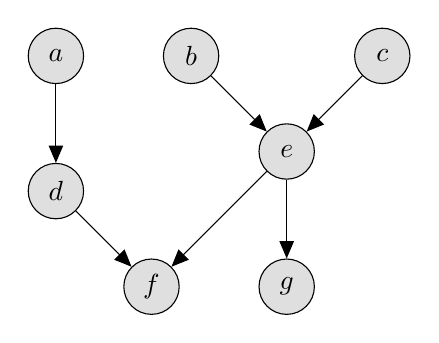
\begin{tikzpicture}
		% Define nodes
		\node[obs]	                 (a)		{$ a $};
		\node[obs, right = of a]	 (b)		{$ b $};
		\node[obs, below right = of b]     (e)     {$ e $}; 
		\node[obs, above right = of e]     (c)     {$ c $}; 
		\node[obs, below = of a]     (d)     {$ d $}; 
		\node[obs, below right = of d]     (f)     {$ f $}; 
		\node[obs, below  = of e]     (g)     {$ g $}; 
		\edge{a}{d};
		\edge{b,c}{e};
		\edge{d,e}{f};
		\edge{e}{g};
	\end{tikzpicture}
	\caption{\label{fig:exBN2}}
\end{figure}
\end{Exercise}

\newpage
		
\subsection{Answers of exercises}

\begin{Answer}[ref=ABC]
We have two categorical variables $A$ and $B$, whose supports are the sets $\mathcal A = \{1, \ldots, n\}$ and $\mathcal B = \{1, \ldots, nm\}$, and we also have a binary variable, whose support is the set $\mathcal C = \{0, 1\}$. The space of joint assignments corresponds to $\mathcal A \times \mathcal B \times \mathcal C$ whose size is $n \times m \times 2$. Therefore, it takes $O(\times n \times m)$ probability values to represent the joint distribution $P_{A,B,C}$.
\end{Answer}

~

\begin{Answer}[ref=cond-ind]

\begin{proof}
\begin{subequations}
\begin{align}
\intertext{From the definition of conditional independence  (\ref{eq:cond-ind})  we know that } 
P(\mathbf X, \mathbf Y| \mathbf Z) &= \underbrace{P(\mathbf X|\mathbf Z) P(\mathbf Y| \mathbf Z)}_{\text{conditional independence}} \\
\intertext{from chain rule, we know that}
P(\mathbf X, \mathbf Y| \mathbf Z) &= \underbrace{P(\mathbf Y|\mathbf Z) P(\mathbf X| \mathbf Z, \mathbf Y)}_{\text{chain rule}} \\
\intertext{if we then replace the left-hand side of the former by the right-hand side of the latter we get}
P(\mathbf Y|\mathbf Z) P(\mathbf X| \mathbf Z, \mathbf Y) &= P(\mathbf X|\mathbf Z) P(\mathbf Y| \mathbf Z) \\
P(\mathbf X| \mathbf Z, \mathbf Y) &= P(\mathbf X|\mathbf Z)
\end{align}
\end{subequations}
\end{proof}

\end{Answer}

~

\begin{Answer}[ref=ABC]
The joint $P_{ABC}$ factorises as below
\begin{equation}
P_{ABC}(a, b, c) = P_A(a)P_{B|A}(b|a)P_{C|B}(c|b)
\end{equation}
and it takes $O(n_a + n_a \times n_b + n_b \times n_c)$ probability values to represent.

The conditional $P_{BC|A}$ is shown below
\begin{subequations}
\begin{align}
P_{BC|A}(b, c|a) &= \frac{P_A(a)P_{B|A}(b|a)P_{C|B}(c|b)}{P_A(a)} \\
 &= P_{B|A}(b|a)P_{C|B}(c|b)
\end{align}
\end{subequations}
where we first applied the definition of conditional probability, and then cancelled the terms $P_A(a)$ that appear both in the numerator and in the denominator.
%Inferring $P_{BC|A}$ takes time $O(n_a \times n_b \times n_c)$ because we have to solve the last equation for all joint outcomes of $B, C|A$.

The conditional $P_{C|A}$ requires can be obtaining by marginalising $B$ out of $P_{BC|A}$, thus we have 
\begin{subequations}
\begin{align}
P_{C|A}(c|a) &= P_{BC|A}(b, c|a) \\
	&=\sum_{b=1}^{n_b} P_{B|A}(b|a)P_{C|B}(c|b)
\end{align}
\end{subequations}
by reusing the result just obtained for $P_{BC|A}$. 
Note that since both terms inside of the sum depend on $B$ (the variable we are marginalising), we cannot further simplify this expression.


\end{Answer}

~

\begin{Answer}[ref=A-G]
The joint distribution factorises as
\begin{equation}
\begin{aligned}
P_{ABCDEFG}(a,b,c,d,e,f,g) &= P_A(a) P_B(b) P_C(c) \\
	&\times P_{D|A}(d|a) \\
	&\times P_{E|BC}(e|b,c) \\
	&\times P_{F|DE}(f|d,e) \\
	&\times P_{G|E}(g|e) 
\end{aligned}
\end{equation}
which takes $O(n_a + n_b + n_c + n_a \times n_d + n_c \times n_b \times n_e + n_e \times n_d \times n_f + n_e \times n_g)$ probability values to represent.
Suppose the worst case where all variables are ``1 of $n$'' for some large $n$, then this takes $O(n^3)$ rather than $O(n^7)$ which would the case had no assumptions been made.
\end{Answer}

For the conditional $P_{FG|ABCDE}$ it's sufficient to recall that the BN chain rule implies that $\mathbf X \perp \text{NonDescendants}_{\mathbf X} \mid \Pa_{\mathbf X}$ for any subset of variables in the network. Thus, if we take the subset $\{F, G\}$, we see that $\Pa_{\{F, G\}} = \{D, E\}$, $\text{NonDescendants}_{\{F, G\}} = \{A, B, C\}$, and then
\begin{subequations}
\begin{align}
P_{FG|ABCDE}(f, g|a,b,c,d,e) &= P_{FG|DE}(f, g|d,e) \\
 &= P_{G|E}(g|e) P_{F|DE}(f|d,e)
\end{align}
\end{subequations}
where the first equality is due to independence on non-descendants $A,B,C$ and the second is due to the factorisation of the BN.
\input{undirected}


\section{Further reading}

\begin{itemize} 
	\item \href{https://homes.cs.washington.edu/~taskar/pubs/gms-srl07.pdf}{Graphical models in a nutshell}
\end{itemize}

\bibliographystyle{apalike}
\bibliography{BIB}

\end{document}
